\documentclass{article}

% Language setting
% Replace `english' with e.g. `spanish' to change the document language
\usepackage[english]{babel}

% Set page size and margins
% Replace `letterpaper' with `a4paper' for UK/EU standard size
\usepackage[a4paper,top=2cm,bottom=2cm,left=3cm,right=3cm,marginparwidth=1.75cm]{geometry}

% Useful packages
\usepackage{amsmath}
\usepackage{graphicx}
\usepackage[colorlinks=true, allcolors=blue]{hyperref}
\usepackage{xcolor}
\usepackage{listings}
\usepackage{multicol}
\colorlet{mygray}{black!30}
\colorlet{mygreen}{green!60!blue}
\colorlet{mymauve}{red!60!blue}

\lstdefinelanguage{cpp}{
  backgroundcolor=\color{gray!10},  
  basicstyle=\ttfamily,
  columns=fullflexible,
  breakatwhitespace=false,      
  breaklines=true,                
  captionpos=b,                    
  commentstyle=\color{mygreen}, 
  extendedchars=true,              
  frame=single,                   
  keepspaces=true,             
  keywordstyle=\color{blue},      
  language=c++,                 
  numbers=none,                
  numbersep=5pt,                   
  numberstyle=\tiny\color{blue}, 
  rulecolor=\color{mygray},        
  showspaces=false,
  showstringspaces=false,
  showtabs=false,                 
  stepnumber=5,                  
  stringstyle=\color{mymauve},    
  tabsize=3,                                     
  title=\lstname 
}
\lstset{language=cpp}
\lstnewenvironment{code}[2][]{%
  \lstset{%
    numbers = left,
    title   = #2,
    #1,
  }%
}{}

\title{Embedded Systems Programming \\ Assignment 3.2 \\ \large Test Driven Development}
\author{Steinarr Hrafn Höskuldsson}

\usepackage{fancyhdr}
\fancypagestyle{firststyle}
{
   \fancyhf{}
   \fancyhead[L]{Embedded Systems Programming}
   
   \renewcommand{\headrulewidth}{0pt} % removes horizontal header line
}

\newcommand{\mycomment}[1]{}
\begin{document}
\pagestyle{firststyle}
{\let\newpage\relax\maketitle}

\mycomment{
\begin{figure}[h]
    \centering
    \includegraphics[width=0.75\textwidth]{LAB3/Basic1.png}
    \caption{"Switch test" Breadboard set up}
    \label{fig:Switch_test}
\end{figure}

\lstinputlisting[caption=main.cpp in Part 3]{Assignment3_1StateBehaviour/src/main_prt3.cpp}

}

\section*{Part 1}
\begin{multicols}{2}
[
A new project was created in PlatformIO and a use case diagram using plantUML was written. 
]
\lstinputlisting[caption=usecase.plantuml]{Assignment3_2TestDrivenDevelopment/docs/diagrams/src/use_case.plantuml}

    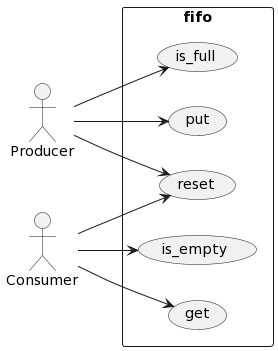
\includegraphics[width=0.5\textwidth]{Assignment3_2TestDrivenDevelopment/docs/diagrams/uscase.png}
    \caption{Use Case Diagram of a First-in-First-out Queue}
\end{multicols}
\\
The test cases were created from the template given in the assignment. The implemented test cases can be seen in Appendix \ref{appendix:test_main.cpp}

\section*{Part 2}
The given templates were copied into the correct positions. \verb!fifo.h! was renamed to \verb!fifo2.h! so it and \verb!fifo2.cpp! could be distinguished from \verb"fifo3.h" and \verb"fifo3.cpp". That way the solutions to Part 2 and Part 3 could be programmed without interfering with each other.

A First-In-First-Out Queue was implemented by using a vector called \verb"buffer" and when an item is 'gotten' the \verb"Fifo" class pops the first item and then moves all the items one step forward. The class keeps count of how many items are in the queue with a private attribute called \verb"count" and therefore knows where to put items that get 'put' to it.


\lstinputlisting[caption=fifo2.cpp - Implementation of a Fifo class using a vector buffer.]{Assignment3_2TestDrivenDevelopment/src/fifo2.cpp}

A main program was written that accepts characters from the Serial port and puts them into the queue. Every second one character is printed from the queue and the onboard LED is turned on while the queue is full. The code for \verb!main.cpp! can be seen in Appendix \ref{appendix:main.cpp}

\section*{Part 3}
A second implementation of the \verb!Fifo! class was written based on a ring buffer. The class uses private attributes \verb"head" and \verb"tail" that are pointers to where in the ring buffer the next item to be 'gotten' is and where the next item to be 'put' should go, respectively.


\lstinputlisting[caption=fifo2.cpp - Implementation of a Fifo class using a ring buffer and pointers.]{Assignment3_2TestDrivenDevelopment/src/fifo3.cpp}
\newpage
\section*{Appendix}
\appendix
\section{Test cases}\label{appendix:test_main.cpp}
\lstinputlisting[caption=Context.h]{Assignment3_2TestDrivenDevelopment/test/test_main.cpp}
\section{main.cpp}\label{appendix:main.cpp}
\lstinputlisting[caption=Context.h]{Assignment3_2TestDrivenDevelopment/src/main.cpp}
\section{Header files}\label{appendix:headers}
\lstinputlisting[caption=Context.h]{Assignment3_2TestDrivenDevelopment/include/fifo2.h}
\lstinputlisting[caption=Context.h]{Assignment3_2TestDrivenDevelopment/include/fifo3.h}
%\lstinputlisting[caption=main.cpp in Part 2]{Assignment3_1StateBehaviour/src/main_prt2.cpp_old}




% TODO: put these in columns next to each other?

\end{document}

